\documentclass[11pt,a4paper]{article}

\usepackage{hyperref}
\usepackage{graphicx}
\usepackage{amssymb}
\usepackage{amsmath}
\usepackage{amsthm}
\usepackage[margin=19mm]{geometry}
\usepackage{natbib}
\usepackage{bm}
\usepackage[toc,page]{appendix}
\usepackage{booktabs}
%\usepackage{url}
%\usepackage{fancyhdr}
%\usepackage{fancyvrb}
\usepackage{lscape}
%\usepackage{pdfsync}
\usepackage{rotating}
\usepackage{multirow}
\usepackage[nodisplayskipstretch]{setspace} \setstretch{1.5}
\let\oldv\verbatim
\def\verbatim{\par\setstretch{0.9}\oldv}
\usepackage[table]{xcolor}
\usepackage{algorithm,algorithmic}

%\renewcommand{\headrulewidth}{0.5pt} %Do not print a rule below the header
%\renewcommand{\footrulewidth}{0pt} %Do not print a rule above the footer

\bibpunct{(}{)}{;}{a}{,}{,}

%\renewenvironment{tabbing}{\linebreak \texttt \sl}{\linebreak}

\newcommand{\undertilde}[1]{\underset{\widetilde{}}{#1}}
\newcommand{\threeScript}[3]{
	\!\begin{smarray}{l}
  		{#1}\\ \hlx{s[-5pt]}
  		{#2}\\ \hlx{s[-5pt]}
  		{#3}
 	 \end{smarray}
}
\renewcommand{\baselinestretch}{1.5}
\setlength{\abovecaptionskip}{5pt}
\setlength{\belowcaptionskip}{-1pt}

\newtheorem{mydef}{Definition}

\floatname{algorithm}{Pseudocode}

\newcommand{\disfrac}{\displaystyle \frac}

\hypersetup{
    bookmarks=true,         % show bookmarks bar?
    unicode=false,          % non-Latin characters in Acrobat’s bookmarks
    pdftoolbar=true,        % show Acrobat’s toolbar?
    pdfmenubar=true,        % show Acrobat’s menu?
    pdffitwindow=false,     % window fit to page when opened
    pdfstartview={FitH},    % fits the width of the page to the window
    pdftitle={My title},    % title
    pdfauthor={Author},     % author
    pdfsubject={Subject},   % subject of the document
    pdfcreator={Creator},   % creator of the document
    pdfproducer={Producer}, % producer of the document
    pdfkeywords={keyword1} {key2} {key3}, % list of keywords
    pdfnewwindow=true,      % links in new window
    linktoc = page,
    colorlinks=true,       % false: boxed links; true: colored links
    linkcolor=blue,          % color of internal links
    citecolor=blue,        % color of links to bibliography
    filecolor=magenta,      % color of file links
    urlcolor=cyan           % color of external links
}

%###################################################################################################
%Writing starts here!!
%
%###################################################################################################

\begin{document}
\title{Introduction}
\author{Kevin Chang}
\date{\today}
\maketitle

%\tableofcontents
%\chapter{Quantitative Proteomics using MudPIT coupled with iTRAQ\textsuperscript{TM}}\label{chap:intro}

\section{Introduction}
Any research study requires the researcher to conduct one or more experiments to make confident claims based on their results. A thorough plan is essential on how an experiment should be conducted is under a particular important aspect of the statistical theory called \emph{experimental design}. 

Much of the initial theory in the experimental design were developed in the field of agricultural by \citep{Fisher1935}. However, the most of these theories were developed with none or very little aid of the computational power; thus, the view in the experimental design today is much differ from that of the 1930s. Therefore, the theory in the experimental design has been developed quite rapidly from the progression of the computers. 
 
The advantages that experimental design can provide is increasing in amount of information per experiment compared to an ad hoc approach. The second benefit is providing an organized approach toward analysis and interpretation of results; thus, facilitating communication between the statistician and the biologist. Another advantage is in the assessment of information reliability in light of experimental and analytical variation \citep{Doyle2009}. 

The type of experiment that this thesis is focusing on is \emph{high-throughput biotechnologies experiment} (HTBE). The HTBE is the testing of multiple samples and each sample with large numbers of candidate molecules, such as genes or proteins, in a biological assay at the same time \citep{Janzen2002}. Having a thorough experimental design becomes particularly important in HTBE, because the cost of these experiments can be very expensive. However, despite high-throughput biotechnologies have improved rapidly within a last decade; the statistical methods, for analysing the data generated from these technologies, are falling further behind \citep{Doyle2009}. Therefore, there is a need to improve in the theory for the design of HTBE. 

There are many different families of designs exits in the published literature such as the reference design or loop design for the microarray experiments. However, most of these HTBE have a two-phase structure, when the responses of experimental units to treatments cannot be measured directly in a single experiment, i.e.\ the gene expression cannot be measured without the use of microarray technology. Thus, subsequent processing (Phase 2) of the initial (Phase 1) experiment is necessary in order for the measurements to be made. An good example is a proteomics experiment, which is the study of proteins. The Phase 1 experiment involves the organisms that are to be perturbed by the experimental conditions of interest. Since the abundance of proteins cannot be measured directly from the organisms, the Phase 2 experiment uses multiplexing techniques such as iTRAQ peptide labelling, coupled with liquid chromatography-mass spectrometry (LC-MS), to measure the abundance of proteins in samples extracted from the organisms in the Phase 1 experiment. Section~\ref{sec:proteomicExpt} describes in detail the biological background of the mass spectrometry based proteomics experiments. 

The purpose of this chapter is to describe how the methods surrounding the two-phase experiments have evolved over the last few decades. 

%This will aid in the understanding of the two-phase experiment which can also be employed as a part of important idea in the designing two-phase experiment.

\section{The introduction of two-phase experiments by McIntyre}
Two-phase experiments were first introduced by \cite{McIntyre1955}, where he discussed an example which came from a real experiment that investigated the effects of four light treatments on the synthesis of tobacco mosaic viruses in the tobacco leaves. In the Phase 1 experiment, two $4 \times 4$ square arrays are made up by eight plants and four leaves within plants. Four different treatments are then assigned to the plants and the leaves within plants in such way where each treatment occurs only once within each row and column in each of two $4 \times 4$ square arrays. This assignment is also known \emph{Latin square design} \citep{Bailey2008}. Hence, there are 32 observations from the Phase 1 experiment. In the Phase 2 experiment, further 16 plants and four leaves within plants were used. In addition, each leaf is further subdivided into two half leaves, which allows to measure 128 samples. Given that there are 32 samples from the Phase 1 experiment, each sample are replicated four times for the measurement in the Phase 2 experiment. For the assignment of the Phase 2 experiment, four $4 \times 4$ square arrays are made up by the 16 plants and four leaves with plants. Furthermore, since each leaf is further subdivided into two half leaves, the Phase 2 design can be expressed as two sets of Latin squares designs superimposed to each other, which also known as  \emph{Greaco-Latin square designs}. To analyse this study, an analysis of variance (ANOVA) table were produced to explain the sources of variation introduced from overall two-phase experiment. For each source of variation, the expected mean squares (EMS), which is the linear combination of variance components, were generated. The \emph{variance component}, commonly denoted by $\sigma_{i}^2$ for factor $i$, indicates the contribution of the variance within each source of variation.  

\citeauthor{McIntyre1955} presented two important principles for designing the two-phase experiment. The replication in the Phase 1 experiment is essential due to the treatment groups are assigned in the Phase 1 experiment. Thus, the statistical test for the treatment effects should be achievable separately from the Phase 2 experiment. The replication in the Phase 2 experiment is not necessary unless there is uncontrollable variation introduced from the Phase 2 experiment. The main objective in the theory of two-phase experiment is the relationship between the factors from the Phase 2 experiment and the Phase 1 experiment. 

(Check!!) For the example experiment mentioned, the replication only applied in the Phase 1 experiment as each sample is replicated four times. 

\citeauthor{McIntyre1955} concluded with three important concepts. Firstly, he demonstrated that the different two-phase design combinations can induce different error variances for the treatment effects, because different designs will result in the different combinations of the variance components. Secondly, based on the example experiment, with doubling in the replication in the Phase 2 experiment, the error variance for the treatment effects is reduced by only $19\%$; however, the amount time for complete the experiment is doubled. Finally, if there is no replication in the Phase 1 experiment, then the error variance for the treatment effects is markedly inflated as it includes the variation between leaves within plants from both Phase 1 and Phase 2 experiments. Therefore, the construction of the ANOVA table with EMS is shown to be essential to illustrate the linear combination of the variance components, especially to estimate the error variance for the treatment effects. However, the method in constructing the ANOVA table with EMS was not mentioned by \citeauthor{McIntyre1955}.
 
\section{Estimation of the treatment and random effects}
Four years later, \cite{Curnow1959} revisits the theory of two-phase experiments. \cite{Curnow1959} produced a new ANOVA table of the overall analysis for \citeauthor{McIntyre1955}’s last example. The new ANOVA table presents every sum of square and the corresponding DF
which shows how the total variation of data from the experiment is separated. In addition, the ANOVA table also shows estimation of the treatment effects is achieved with the variance components of between leaves from Phase 1 and 2 experiments, i.e.\ sums analysis, or is achieved with the variance component of between leaves from the Phase 1 experiment only, i.e.\ differences analysis. 


McIntyre used Latin square analysis to estimate the treatment effect which is equivalent of taking the un-weighted estimate the treatment effects. However, based on the new ANOVA table presented, the sums and differences analyses are equivalent of inter-block and intra-block analyses, respectively, that are arise in the analysis of an incomplete block design. If the variances in the treatment estimates from the inter-block and intra-block analyses are very different, then Curnow believed that weighting the estimates according to treatment variances would be a better method. Thus, the treatment estimate is given by 
\begin{equation}\label{eq:weightTrtEst}
\hat{\tau} = w \hat{\tau}_{inter} + (1 - w)\hat{\tau}_{intra} ,
\end{equation}
where $w$ denotes the weight, and $\overline{\tau}_{inter}$ and $\overline{\tau}_{intra}$ denotes the treatment estimates from the inter-block and intra-block analyses, respectively. Since the variance of treatment estimate can be expressed as 
\[
\mathrm{Var}[w  \hat{\tau}_{inter} + (1 - w)\hat{\tau}_{intra}] = w^2 \mathrm{Var}(\hat{\tau}_{inter}) + 2 w (1-w)  \mathrm{Cov}(\hat{\tau}_{inter}, \hat{\tau}_{intra}) + (1-w)^2 \mathrm{Var}(\hat{\tau}_{intra}), 
\]
which is minimised by choosing 
\begin{equation}
w = \frac{\mathrm{Var}(\hat{\tau}_{intra}) - \mathrm{Cov}(\hat{\tau}_{intra}, \hat{\tau}_{inter})}{\mathrm{Var}(\hat{\tau}_{intra}) + \mathrm{Var}(\hat{\tau}_{inter}) - 2\mathrm{Cov}(\hat{\tau}_{intra}, \hat{\tau}_{inter})}.
\end{equation}

For the variance components present in the intra-block and inter-block analyses, \cite{Curnow1959} also used the weighted estimates by combining the variance component estimates from these two analyses. The weight is also computed by minimising the variances of the variance component estimate.

However, for the example given by McIntyre, the \citeauthor{Curnow1959}'s method did not produce a very different estimation for both treatment effects and the variance components comparing to \cite{McIntyre1955}. Nevertheless, the new ANOVA table, given by  \cite{Curnow1959},emphasised in the combining the estimates from the intra-block and inter-block analyses which provides a first improvement in developing a better analytic procedure for the two-phase experiments. 


\section{Further development in the two-phase experiment theory}
Since the initial introduction of two-phase experiments by \citeauthor{McIntyre1955} and subsequent investigation by \citeauthor{Curnow1959}, there was no attention given to this theory until by \cite{Brien1983}. 

So far both paper did not mention on how the ANOVA table is constructed 


Two sets of steps were described, the first set is to determine the overall structures of the experiment and the second set is to derive the ANOVA table based on the experimental structure.

To determine the overall structures of the experiment

First step is to identify the factors associated the experimental and observational units.

Second step is to group the factors to form the tier. 


To describe his method briefly, first step is to identify the factors associated the experimental and observational units, then group these factors into different sets, called \emph{tiers}. (Defined these)


The last step is to determine the relationship between the factors within each tier. using the syntax



He proposed a set of rules for deriving the ANOVA table with sources of variation and degrees of freedom.

First step is to expand the structure formula for each tier.

Each expanded term in the first tier will have a line to initialise the ANOVA table.

Each expanded term from the second tier will be include in the table under the terms of the first tier. The terms from the second tier are shown as indented in the ANOVA table to differentiate from the terms in the first tier. 

The residual lines are included for any excess informtaion of the confounded terms. 
















For the two-phase experiment, there will be at least three tiers of factors, two set of block factors and one set of treatment factors. Hence, two-phase experiments also known as \emph{multi-tiered experiment}. The tier 1 and 2 consist of block factors of the Phase 2 and 1 experiments, respectively. The third tier is then contain the treatment factors of the overall experiments.  

To derive the ANOVA table, first step is to expand the structure formulae for each tier using the \citeauthor{Wilkinson1973}'s syntax. The expansion of the first tier structure formula generates a set of terms that is used to construct the ANOVA table. The next step is to examine for any terms of higher tiers that is confounded with terms in the lower tiers. For example, if a term from tier 2 is confounded with a term from tier 1, then this tier 2 term should be underneath the tier 1 term with indentation in the ANOVA table. 

The presence of confounding can be determined by study the contrasts that associated specific factors. For example, if a factor from a lower tier is confounded with another factor from a higher tier, then this factor of the lower tier should be in the stratum of that factor from the higher tier in the ANOVA table. For a more detail description of these procedures see \cite{Brien1983}.

\cite{Brien1983} also acknowledged the randomisation procedures in between the factors of tiers can affect the relationship of factors within each tier. Consider an experiment with row-column design, thus the relationship between the row and column factor is thought to be crossed.  If the treatment factor is randomised only to the column factor, then the treatment is not orthogonal to the column within each row. Thus, the relationship between the row and column is then becomes nested. More on the randomisation of two-phase experiment is given in \cite{Brien2006b}.

\section{Symbolic syntax represent the structure formula}
\cite{Wilkinson1973} developed a symbolic syntax for representing the relationship between the block factors (i.e. block structure) and treatment factors (i.e. treatment structure) in an experiment. \cite{Brien1999} referred to this representation as a \emph{structure formula}. \citeauthor{Wilkinson1973}'s syntax was originally developed to generate and analyse the ANOVA models in the GenStat statistical analysis program, although it is now widely used in many statistical packages. Two basic operations for representing block and treatment structures, namely \emph{crossing} and \emph{nesting}, will be described. 

Both relationships are described using the basic single-phase experiment examples.

Using these two relationships helps in constructing the linear model of the experiment.  

\subsection{Crossing}\label{subsec:cross}
A factorial experiment involves two or more treatment factors, such that the levels of every treatment factor occur together. Hence, the analysis of factorial experiments consists of main effects, the effects of each treatment factor separately, and interaction effects, the effects of every combination of the levels of the different treatment factors. \citeauthor{Brien1999}'s paper provided an example of such an experiment involving two treatment factors, namely trellising and pruning methods.

Consider a basic factorial linear model for two factors, A and B, written as
\begin{equation}\label{eq:crossModel}
y_{ij}= \mu + a_{i} + b_{j} + (ab)_{ij},
\end{equation}
\begin{center}
($i=1,\dots ,t$; $j=1,\dots,r$)
\end{center}
where $y_{ij}$ denotes the observation for the $(ij)$th factorial treatment combination, $\mu$ denotes the grand mean, $a_{i}$ and $b_{j}$ denote the main effects of factors A and B at levels $i$ and $j$, respectively, and $(ab)_{ij}$ denotes the interaction between factor A at level $i$ and factor B at level $j$. The linear model in~(\ref{eq:crossModel}) is also appropriate for experiments in which two block factors are crossed, as is the case for row-column designs. Then, the $(ab)_{ij}$ denotes the error term of the row-column block structure model. 

The Wilkinson and Rogers syntax representation of the factorial treatment structure in~(\ref{eq:crossModel}) is
\[
A*B,
\]
where `$*$' denotes the \emph{crossing} of factors A and B. This treatment structure statement is expanded to its elementary form
\begin{equation}\label{eq:expandCross}
A + B +A\cdot B,
\end{equation}
involving only the operators `$+$', denoting the sum of the model terms, and `$\cdot$', linking the individual factors to multi-factor terms. In this case, $A$ and $B$ denote the main effects of factors A and B, respectively, and $A\cdot B$ denotes the interaction. Hence, $A$, $B$ and $A\cdot B$ correspond to the terms $a_{i}$, $b_{j}$ and $(ab)_{ij}$, respectively, in model~(\ref{eq:crossModel}).

An alternative to the expansion shown in~(\ref{eq:expandCross}) is to use an approach which satisfies algebraic multiplication. To achieve this, the identity term, $I$, is included in the structure formula. Hence, the terms in~(\ref{eq:expandCross}) are redefined as $A=I+A'$ and $B=I+B'$, where `$'$' is used to distinguish the new term, $A'$, in the algebraic model from original term, $A$, in the structure formula~(\ref{eq:expandCross}). Then, structure formula~(\ref{eq:expandCross}) can be rewritten and expanded as
\begin{equation}\label{eq:expandCross2}
(I + A')(I + B') = I + A' + B' + A'B',
\end{equation}
where the resultant $I$ denotes the grand mean, $A'$ and $B'$ denote the main effects of factors A and B, respectively, and $A'B'$ denotes their interaction. Hence, the result from the algebraic multiplication provides an one-to-one correspondence between the terms in the linear model in~(\ref{eq:crossModel}) and the terms on the right hand side of the equation in~(\ref{eq:expandCross2}). Furthermore, each term in both~(\ref{eq:crossModel}) and~(\ref{eq:expandCross2}) corresponds to a source of variation in the factorial experiment.

Equation~(\ref{eq:expandCross2}) now provides a straightforward method for deriving the DF associated with each source of variation in the factorial experiment. Suppose, in the above example, that factors A and B have $n_A$ and $n_B$ levels, respectively, and the grand mean has only one level. Then, the DF associated with main effects of A and B are $n_A - 1$ and $n_B - 1$, respectively. This is due to each factor having its own parameter space with a specific dimension. To estimate the effect of each factor of the model, the grand mean needs to be adjusted or swept for every factor. As result, the DF of the effects A and B are the difference of the dimensionalities in parameter spaces between the main effects and the grand mean, i.e. $n_A - 1$ and $n_B - 1$ \citep{Good1973}. Furthermore, the DF associated with the interaction is $(n_A - 1)(n_B - 1)$. There is also one DF associated with the grand mean. This leads to the \emph{DF identity} of the cross model~(\ref{eq:crossModel}), written as 
\begin{equation}\label{eq:crossDF}
1 + (n_A - 1) + (n_B - 1) + (n_A - 1)(n_B - 1).
\end{equation} 

To further elaborate the cross model in~(\ref{eq:crossModel}), the \emph{yield identity} can also be used to explain the effects of each factor in liner model in~(\ref{eq:crossModel}). \cite{Nelder1965A} had given a guideline to derive the yield identity from the DF identity. The terms of the DF identity given in~(\ref{eq:crossDF}) are first expanded as
\begin{equation}\label{eq:crossExpandDF}
1 + (n_A - 1) + (n_B - 1) + (n_A n_B - n_A - n_B + 1),
\end{equation} 
where the numeric value $1$ corresponds to the grand mean and the other terms correspond to the averages of the the $y's$ over the missing suffices of the terms in~(\ref{eq:crossExpandDF}). For example, since the suffix of factor B is absent in $n_A$, this term corresponds to the $\displaystyle \frac{\sum_{j=1}^t y_{ij}}{t}$. However, the term $n_A n_B$ contains the suffices of both factors A and B, so this term corresponds to $y_{ij}$. Hence, the yield identity is written as
\begin{equation}\label{eq:crossYield}
y_{ij} \equiv \bar{y}_{..} + (\bar{y}_{i.} - \bar{y}_{..}) + (\bar{y}_{.j} - \bar{y}_{..}) +(y_{ij} - \bar{y}_{i.} - \bar{y}_{.j} + \bar{y}_{..}),
\end{equation}
where $\equiv$ denotes the equivalence relation, the dot of the suffices denotes the summation over the subscript which is replaced and the over-line indicates the average over the terms associated with the nominal subscript. Thus, $\bar{y}_{..}$ denotes the grand mean of all observations, $\bar{y}_{i.}$ and $\bar{y}_{i.}$ are the means of the observations for factor A at level $i$ and factor B at level $j$, respectively. Each set of terms, contained within parentheses, of the yield identity in~(\ref{eq:crossYield}) is an estimate of the effect for a source of variation and corresponds to a specific factor in equation~(\ref{eq:crossModel}).

The matrix notation of the cross model in~(\ref{eq:crossModel}) can also be written which had shown to have a more clear characteristic of the yield identities in~(\ref{eq:crossYield}) \citep{Nelder1965A}. The first term  in~(\ref{eq:crossYield}), $y_{ij}$, corresponds $\bm{y}$ denote the vector of responses,
\[
(y_{11}, y_{12}, \dots, y_{1r}, y_{21}, \dots, y_{tr}) 
\]
The grand mean, $\bar{y}_{..}$, can be computed by pre-multiply an averaging matrix, denotes by $K_{tr}$, to the vector of responses, $\bm{y}$. This \emph{averaging matrix}, $K_{tr}$, is a square matrix of order $tr$ with all elements equal $\frac{1}{tr}$. For the terms $\bar{y}_{i.}$ and $\bar{y}_{.j}$, since these two terms compute the averages over $j$ and $i$ respectively, thus, the square matrices that used to pre-multiply the $\bm{y}$ are $I_{t} \otimes K_{r}$ and $K_{t} \otimes I_{r}$, respectively, where $I$ denotes the \emph{identity matrix} and $\otimes$ denotes \emph{Kronecker product}. Therefore, the matrix notation of the yield identity in~(\ref{eq:crossYield}) is written as 
\begin{equation}\label{eq:crossYieldMatrix}
\bm{y} = K_{tr}\bm{y} + (I_{t} \otimes K_{r} - K_{tr})\bm{y} + (K_{t} \otimes I_{r} - K_{tr})\bm{y} + (I_{tr} - I_{t} \otimes K_{r} - K_{t} \otimes I_{r} + K_{tr})\bm{y}.
\end{equation}

In summary, Table~\ref{tab:expandCross} presents the association of each source of variation to the DF, each term in linear model~(\ref{eq:crossModel}), the structure formula in~(\ref{eq:expandCross2}) and the yield identity in both linear and matrix forms in~(\ref{eq:crossYield}) and (\ref{eq:crossYieldMatrix}), respectively.

\subsection{Nesting}
Consider a group of experimental units which form a block, these experimental units, namely plots, are said to be nested within that block. \citeauthor{Brien1999}'s paper also provides an example of such a structure in the phase 1 viticultural experiment, where the four columns are nested within each of the two square blocks.

More generally, consider a field experiment consisting of $n_A$ blocks each containing $n_B$ plots. Let $y_{ij}$ denote the observation on the $j$th plot within block $i$. Then, the linear model for a basic nested design with the levels of the plot factor $B$ nested within the block factor $A$ is given by
\begin{equation}\label{eq:nestModel}
y_{ij}= \mu + a_{i} + (ab)_{ij},
\end{equation}
where $\mu$ denotes the grand mean, $a_{i}$ denotes the main effect of $i$th block, and $(ab)_{ij}$ denotes the effect of the $j$th plot within block $i$. The term $(ab)_{ij}$ in~(\ref{eq:nestModel}) represents the variation between plots with a same block and is generally denoted by $\epsilon_{ij}$. This is also known as a \emph{null experiment} where the treatment information is not included in the analysis.

The Wilkinson and Rogers syntax for representing the nested block structure in~(\ref{eq:nestModel}) is
\begin{equation} \label{eq:simpleNest1}
A/B,
\end{equation}
where `$/$' denotes the nesting of the levels of factor B within the levels of factor A. The expansion of the structure formula in~(\ref{eq:simpleNest1}) to its elementary form is then
\begin{equation}\label{eq:simpleNest2}
A + A\cdot B,
\end{equation}
where $A$ denotes the main effect of factor A and $A\cdot B$ denotes the effects of the levels of factor B nested within the levels of factor A. This is different to the elementary form of two crossed factors in~(\ref{eq:expandCross}) which includes a term for the main effect of factor B and where $A\cdot B$ denotes interaction effect. The elementary form of the basic nested block design in~(\ref{eq:simpleNest2}) does not contain the main effect of factor B because it is absorbed into the term $A\cdot B$. This can be shown when the structure formula is re-expressed algebraically later. Note that the terms $A$ and $A\cdot B$ in~(\ref{eq:simpleNest2}) correspond to the terms $a_{i}$ and $(ab)_{ij}$, respectively, in model~(\ref{eq:nestModel}).

The structure formula in~(\ref{eq:simpleNest2}) can be rewritten and expanded using algebraic multiplication by including the identity term, $I$, as described in Subsection~\ref{subsec:cross}. Firstly, let $A = I+A'$ and $B = I+B'$. The nesting operator is then treated as multiplication, i.e.
\[(I + A')/(I + B') = I + A'+ (I + A')B'.\]
If the term $(I + A')B'$ is expanded
\[I + A')B' = B' + A'B' \]
where $B'$ denotes the effect of factor B and $A'B'$ denotes the interaction between factors A and B. However, these two effects cannot stand alone because they together contribute to the effect of between plots within a block. This nested structure will be denoted by defining $\overline{A}=I+A'$, which gives the final expression
\begin{equation}\label{eq:expandSimpleNest}
I + A'+ \overline{A}B'.
\end{equation}

The next step is to derive the DF associate with each source of variation in~(\ref{eq:expandSimpleNest}). There are $n_A - 1$ DF associated with the $A'$ main effect. However, the DF associated with the $\overline{A}B'$ is $n_A (n_B - 1)$, because $\overline{A} = I + A'$, thus, the DF is $1 + (n_A - 1) = n_A$. Hence, the DF identity of the nested model in~(\ref{eq:simpleNest1}) is 
\begin{equation}\label{eq:simpleNest1DF}
1 + (n_A - 1) + n_A(n_B - 1).
\end{equation}

Using the method mentioned in subsection~\ref{subsec:cross}, from the DF identity, the yield identity can be derived as
\begin{equation}\label{eq:simpleNestYield}
y_{ij} \equiv \bar{y}_{..} + (\bar{y}_{i.} - \bar{y}_{..}) + (y_{ij} - \bar{y}_{i.}).
\end{equation}
It follows by the the matrix notation of the yield identity similar to~(\ref{eq:crossYieldMatrix}) as 
\begin{equation}\label{eq:simpleNestYieldMatrix}
\bm{y} = K_{tr}\bm{y} + (I_{t} \otimes K_{r} - K_{tr})\bm{y} + (I_{tr} - I_{t} \otimes K_{r})\bm{y}.
\end{equation}

In summary, Table~\ref{tab:expandSimpleNest} presents the association of each source of variation to the DF, each term in linear model~(\ref{eq:nestModel}), the structure formula in~(\ref{eq:expandSimpleNest}) and the yield identity in both linear and matrix forms in~(\ref{eq:simpleNestYield}) and (\ref{eq:simpleNestYieldMatrix}), respectively.



\subsection{Complicated Nesting Structure}
Consider now another block structure consisting of three factors, $A$, $B$ and $C$, nested within one another. Let $y_{ijk}$ denotes the observation on the $k$th half-plot within the $j$th plot within block $i$. Then, the linear model for this nested design with the levels of the half-plot factor, $C$, nested within the levels of the plot factor, $B$, nested within the levels of the block factor, A, is given by
\begin{equation}\label{eq:complexNestModel}
y_{ijk}= \mu + a_{i} + (ab)_{ij} + (abc)_{ijk},
\end{equation}
where the last term, $(abc)_{ijk}$, denotes the effect of $k$th half-plot within the $j$th plot within block $i$ and where the remaining terms were defined in~(\ref{eq:nestModel}) of the basic nested design.

The block structure formula can be written as
\begin{equation}\label{eq:complexNest2}
A/B/C
\end{equation}
and the expansion follows the left-to-right rule described by \cite{Wilkinson1973}, giving
\begin{equation}\label{eq:expandComplexNest2}
(A + A\cdot B)/C = A + A\cdot B + A\cdot B\cdot C.
\end{equation}

Structure formula~(\ref{eq:complexNest2}) is now rewritten and expanded using algebraic multiplication. Firstly, the terms in~(\ref{eq:complexNest2}) are substituted with $A = I + A'$, $B = I + B'$ and $C = I + C'$, giving
\begin{equation}\label{eq:expandedNest1}
(I + A')/(I+ B')/(I + C').
\end{equation}
Following the left-to-right rule, $(I + A')/(I+ B')$ is first expanded using the result from basic nested design in~(\ref{eq:expandSimpleNest}). Equation~(\ref{eq:expandedNest1}) is then further expanded as
\begin{equation*}
(I + A'+ \overline{A}B')/(I + C') = I + A'+ \overline{A}B' + (I + A'+ \overline{A}B')C'.
\end{equation*}
Substituting $\overline{A}$ inside the parentheses with $I + A'$, the terms inside the parentheses can be factorised as follow
\begin{eqnarray}
\nonumber&&I + A'+ \overline{A}B' + (I + A'+ (I + A')B')C'\\
\nonumber&=& I + A'+ \overline{A}B' + (I + A'+ B' + A'B')C'\\
\nonumber&=& I + A'+ \overline{A}B' + (I + A')(I+ B')C'\\
\label{eq:expandedNest} &=& I + A' + \overline{A}B' + \overline{A}\overline{B}C',
\end{eqnarray}
where $\overline{A} = I + A'$ and $\overline{B} = I+ B'$, $I$ denotes the grand mean, $A'$ denotes the main effect of factor A, $\overline{A}B'$ denotes the effect of factor B nested within factor A, and $\overline{A}\overline{B}C'$ denotes the effect of factor C nested within factors A and B. 

Using the method mentioned in subsection~\ref{subsec:cross}, from the DF identity, the yield identity can be derived as
\begin{equation}\label{eq:simpleNestYield}
y_{ijk} \equiv \bar{y}_{...} + (\bar{y}_{i..} - \bar{y}_{...}) + (\bar{y}_{ij.} - \bar{y}_{i..}) + (\bar{y}_{ijk} - \bar{y}_{ij.}).
\end{equation}
It follows by the the matrix notation of the yield identity similar to~(\ref{eq:crossYieldMatrix}) as 
\begin{equation}\label{eq:simpleNestYieldMatrix}
\bm{y} = K_{trv}\bm{y} + (I_{t} \otimes K_{rv} - K_{trv})\bm{y} + (I_{tr} \otimes K_{v} - I_{t} \otimes K_{rv})\bm{y} + (I_{trv} -I_{tr} \otimes K_{v})\bm{y}.
\end{equation}

Each of these terms corresponds to a source of variation in the ANOVA. The DF for term in~(\ref{eq:expandedNest}) and the one-to-one correspondence between each of these terms and those in the linear model in~(\ref{eq:complexNestModel}) are presented in Table~\ref{tab:expandComplexNest}.

\begin{landscape}
\begin{table}[ht]
\caption{Correspondence between the terms in the linear model for each source of variation in a basic factorial experiment}
\centering
\begin{tabular}{lccccr}
\hline
\multicolumn{1}{l}{Source of Variation} & \multicolumn{1}{c}{Linear} & \multicolumn{1}{c}{Structure}  & \multicolumn{1}{c}{DF}& \multicolumn{1}{c}{Yield identity}& \multicolumn{1}{c}{Yield identity}\\
\multicolumn{1}{l}{} & \multicolumn{1}{c}{model} & \multicolumn{1}{c}{formula}  & \multicolumn{1}{c}{}& \multicolumn{1}{c}{(linear form)}& \multicolumn{1}{c}{(matrix form)}\\
\hline
Grand mean 				 &$\mu$		  &$I$		& 1 					&$\bar{y}_{..}$ 			&$K_{tr}\bm{y}$\\
Main effect of factor A  &$a_i$ 	  &$A'$		&$n_A - 1$ 				&$\bar{y}_{i.} - \bar{y}_{..}$ 
						 &$(I_{t} \otimes K_{r} - K_{tr})\bm{y}$\\
Main effect of factor B  &$b_j$ 	  &$B'$		&$n_B - 1$ 				&$\bar{y}_{.j} - \bar{y}_{..}$ 
						 &$(K_{t} \otimes I_{r} - K_{tr})\bm{y}$\\
Interaction, AB 		 &$(ab)_{ij}$ &$A'B'$	&$(n_A - 1)(n_B - 1)$   &$y_{ij} - \bar{y}_{i.} - \bar{y}_{.j} + \bar{y}_{..}$ 			 &$(I_{tr} - I_{t} \otimes K_{r} - K_{t} \otimes I_{r} + K_{tr})\bm{y}$\\
\hline
\end{tabular}
\label{tab:expandCross}
\end{table}
\begin{table}[h!]
\centering
\caption{Correspondence between the terms in the linear model for each source of variation in a basic nested experiment}
\begin{tabular}{lccccr}
\hline
\multicolumn{1}{l}{Source of Variation} & \multicolumn{1}{c}{Linear} & \multicolumn{1}{c}{Structure}  & \multicolumn{1}{c}{DF}& \multicolumn{1}{c}{Yield identity}& \multicolumn{1}{c}{Yield identity}\\
\multicolumn{1}{l}{} & \multicolumn{1}{c}{model} & \multicolumn{1}{c}{formula}  & \multicolumn{1}{c}{}& \multicolumn{1}{c}{(linear form)}& \multicolumn{1}{c}{(matrix form)}\\
\hline
Grand mean 					& $\mu$ & $I$	 & 1 & $\bar{y}_{..}$ & $K_{tr}\bm{y}$\\
Block effect of factor A 	& $a_i$ & $A'$	 	& $n_A - 1$ & $\bar{y}_{i.} - \bar{y}_{..}$ & $(I_{t} \otimes K_{r} - K_{tr})\bm{y}$\\
Plot effect of factor B 	& $(ab)_{ij}$ & $\overline{A}B'$	 & $n_A (n_B - 1)$ & $y_{ij} - \bar{y}_{i.}$ & $(I_{tr} - I_{t} \otimes K_{r})\bm{y}$\\
\hline
\end{tabular}
\label{tab:expandSimpleNest}
\end{table}

\begin{table}[h!]
\centering
\caption{Correspondence between the terms in the linear model for each source of variation in the complex nested experiment}
\begin{tabular}{lccccr}
\hline
\multicolumn{1}{l}{Source of Variation} & \multicolumn{1}{c}{Linear} & \multicolumn{1}{c}{Structure}  & \multicolumn{1}{c}{DF}& \multicolumn{1}{c}{Yield identity}& \multicolumn{1}{c}{Yield identity}\\
\multicolumn{1}{l}{} & \multicolumn{1}{c}{model} & \multicolumn{1}{c}{formula}  & \multicolumn{1}{c}{}& \multicolumn{1}{c}{(linear form)}& \multicolumn{1}{c}{(matrix form)}\\
\hline
Grand mean 					& $\mu$ & $I$	 & 1 & $\bar{y}_{..}$ & $K_{tr}\bm{y}$      \\
Block effect of factor A 	& $a_i$ & $A'$	 	& $n_A - 1$ & $\bar{y}_{i..} - \bar{y}_{...}$  & $(I_{t} \otimes K_{rv} - K_{trv})\bm{y} $  \\
Plot effect of factor B 	& $(ab)_{ij}$ & $\overline{A}B'$	 	& $n_A (n_B - 1)$ & $\bar{y}_{ij.} - \bar{y}_{i..}$ & $(I_{tr} \otimes K_{v} - I_{t} \otimes K_{rv})\bm{y}$ \\
Half-plot effect of factor C 	& $(abc)_{ijk}$ & $\overline{A}\overline{B}C'$	 	& $n_A n_B (n_C-1)$ & $\bar{y}_{ijk} - \bar{y}_{ij.}$ & $(I_{trv} -I_{tr} \otimes K_{v})\bm{y}$ \\
\hline
\end{tabular}
\label{tab:expandComplexNest}
\end{table}
\end{landscape}

More generally, let $M$ denote a single factor and $L$ denote either a single or multiple factors. Then, for factor $M$ nested within factor(s) $L$, i.e.
\begin{equation*}
L/M = L + \mathrm{FAC}(L) \cdot M,
\end{equation*}
where $\mathrm{FAC}(L)$ is the dot product of all factors represented by $L$ \citep{Wilkinson1973}.

Thus, the model structure syntax not only allows us to represent a complex model with nesting and crossing relationships, it also allows us to decompose the information into different sources of variation. Then, the DF associated with each source of variation can be derived by expanding the structure formula into its elementary form. Finally, the DF identities are used to deduce the linear and matrix forms of the yield identities, which gives a better clarification of each terms in the linear model. For further detail see \cite{Wilkinson1973} and \cite{Nelder1965A}.



\section{Non-orthogonal block structure}
\cite{Wood1988} emphasised the importance of studying the non-orthogonal block structure in analysing the two-phase experiments. They defined the orthogonal block structure from Houtman and Speed (1983) is that the variance of the data, denoted by $V$, consists of a matrix having the form of 
\begin{equation} \label{eq:varData}
V = \sum_{i} \xi_i P_i
\end{equation}
where  $\xi_i$ associated with the EMS and $P_i$ is a set of known matrices that are orthogonal to each other, i.e. the product of any two matrices equals to zero. If the block structure is non-orthogonal, then at least one pair of matrices in $P_i$ will not be non-orthogonal. Equation~\ref{eq:varData} is discuss more detail in Chapter~2 of this thesis. 

\cite{Wood1988} described how the equation~\ref{eq:varData} can be modified for the two-phase experiments. The two-phase experiment comprised of two sets of block structures from Phase 1 and Phase 2 experiments; thus, the variance of data can be written as 
\begin{equation}
V = \sum_{i} \xi1_i P1_i + \sum_{j} \xi2_j P2_j
\end{equation}
where the two sums denote the block structure from the Phase 1 and Phase 2 experiments, respectively. If the block structure is non-orthogonal, then the products from the pairs of matrices in  $P1_i$ and $P2_i$ should be non-orthogonal. (Need to check). 

The efficiency factor is the amount of treatment information presents for the intra-block analysis \citep{Yates1936}. The artificial example presented shows the efficiency factor for Phase 1 block factors can also be computed when the assignment of Phase 1 units to the Phase 2 blocks is non-orthogonal. 

 were used to compute the treatment estimators and generalized least squares estimators which is an extension from the method described by \cite{Curnow1959}. 

Focusing only on the relationship between the treatment and the Phase 2 experiment, the combine treatment estimates is identical to Equation~\ref{eq:weightTrtEst}. However, the weight becomes
\begin{equation} \label{eq:weightWood}
\frac{(1 - E_\tau)\xi_{intra}}{(1 - E_\tau)\xi_{inter} + E_\tau \xi_{intra}},
\end{equation}
where $E_\tau$ denote the efficiency factor for the amount of treatment information in the intra-block analysis, $\xi_{inter}$ and $\xi_{intra}$ are variance component estimates from the inter and intra-block of Phase 2 experiment, respectively. 

\cite{Wood1988} then showed the optimal weights for estimating the treatment effects are depending on the treatment efficiency factor with respect to the Phase 2 block structure and the variance components from the Phase 2 experiments. Only the variance of the treatment effect estimates is shown to depend on the variance components of Phase 1 experiment. Therefore, they concluded the experimental design should be chosen based on the second phase design where the treatment information is maximised for the intra-block analysis.

In practice, the variance components, from the non-orthogonal block design of two-phase experiments cannot be estimated unless using some computationally intensive methods. Instead, \cite{Wood1988} noted the idea of using restricted maximum likelihood (REML), described by \cite{Patterson1971}, to obtain these variance component estimates. 

 


\section{Viticultural experiment}
\cite{Brien1999} described a viticultural experiment which has a two-phase structure. They then described an algorithm consists of fitting terms in the model by a series of sweeping operations for decomposing the two-phase experiment. 

There are two types of sweeping operations originally discussed by \cite{Wilkinson1970} and \cite{Payne1977}. The first type of sweep is the \emph{pivotal sweep} which involves the effects that are placed into a unit length vector. In another words, this sweep is projecting the data vector from one space to another space. The space is corresponding to the each term expand from the structure formula. Thus, this sweeping operator can be express as 
\begin{equation}
E_i P_i
\end{equation}
where $E_i$ and $P_i$ are the efficiency factor and projection matrix associated with the term $i$ from the expanded structure formula. 

The second type of sweep is called \emph{reanalysis sweep}; which is performed when terms from two different structure formulae are non-orthogonal to each other. Before sweeping to the next term, this effect is removed using the reanalysis sweep. The sweeping operator can be express as 
\begin{equation}
I - E_i P_i
\end{equation}
where $I$ is the identity matrix. Thus, the reanalysis sweep is generally performed after the pivotal sweep. Utilising these two sweeping sequences will allow the computation of the sum of square in the ANOVA table. 







\section{Plant experiment examples}
A series of plant breeding experiments using two-phase experiment were published since then. A series of plant breeding experiments using two-phase experiment were published since then. \cite{Willis2000} investigated the causes of non-indigenous invader plant grows taller and whether it is associated with the genetic level or environmental level. The first phase experiment involves the collection of seeds and the second phase includes the experimental layout of the seedling in the field. The author used the analysis of covariance (ANCOVA) to analyse the data. Due to the missing observations in the experiment, the REML analysis was also conducted to investigate whether the ANCOVA results were biased by the missing data. The results are both methods were shown to be very similar. This study found a little evidence that increased plant size is a genetically determined characteristic of invasive plants.
  
\cite{Smith2001} investigated the genetic mapping of milling yield in wheat using the two-phase experiment. The first phase is a field experiment which the plant materials consist of double haploid line from two mapping populations in a randomised complete block design. One of two populations was divided into two subsets, and the analysis was performed on each of three populations. The grain sample from the field plots were processed for the subsequent second phase. The authors used resolvable incomplete block design and neighbour balanced design for two of three different sets of samples. The author discussed how the linear model and ANOVA table were built. REML was also used in this study to estimate the variance parameters. In their discussion, authors stated further research is required to provide an efficient arrangement of the sample in the field and in the laboratory with adequate replication in both phases.

\cite{Cullis2003} presented a barely malting quality experiment, which is a three-phase experiment. In their study, there were three different sets of data available from three different field trails. The first two were completed in 2000 and used un-replicated grid plot design with a single plot for each doubled haploid line and multiple plots of Arapiles and Franklin arranged in a systematic grids throughout the trial. The trial in 2001 was designed as randomised complete block design with neighbour balance. Each trial was tested separately in the laboratory for the second phase experiment using a randomised block design. These samples were further processed in order to obtain the traits of interest. This phase involves analysing samples in batches which is a nested block design. Hence, this study consists of three phases: the field trial, malting phase and the analysis of starch enzymes in batches. The author followed the methods described in \cite{Brien1983} to classify the linear mixed model, structure formulae and ANOVA table for this three-phase experiment. REML was again used to estimate the variance components. The result showed the presence of both field spatial and laboratory variation in the experiment. In the discussion, the author emphases a need for developing standard designing software that generates an efficient two-phase design which account for both field spatial and laboratory variation. 
 	
\cite{Smith2006} published a simulation study based on a plant breading and genetic mapping experiment to show the benefits of using the two-phase experimental design. The authors proposed a general linear mixed model that removes any restriction concerning orthogonality of block structure. A new design principle was proposed namely p/q-rep design, where p is the proportion of Phase 1 replicates to the genotypes and q is the proportion of the Phase 2 replicates to the Phase 1 replicates. This study shows that p=q=0.1 was better than the experiment without replication. The study also shows using phase 2 replication always had higher realized genetic gain that those did not, which conclude the Phase 2 replication is essential for the genetic mapping experiment. There was not any spatial correlation was shown in the phase 1 experiment, which indicating replication in the first phase is not as essential. 

\section{Moving toward a high-throughput biotechnology }
\cite{Jarrett2008} looked at the two-phase experiment for gene expression two-colour microarray. Initially, they discussed the different orders of fitting the factors to the model can affect the structure of ANOVA table and the way to analyse the treatment effects i.e.\ computing the F-ratio.

Two different types of designs were investigated, these were multiple dye-swap and alternating loop designs. The result shows the multiple dye-swap design is a more robust method, because there are always have at least (r-1) DF for estimating the variance for treatment comparisons. REML was again shown to be a better approach to estimate the variance components. The effectiveness of the estimate was assessed using the effective degrees of freedom computed by the first two moments of an approximating chi-square distribution.

\section{Work by Brien and Bailey} 
Brien and Bailey have done more extensive work on the two-phase experiments. \cite{Brien2006b} describes the multiple randomisations that involves with the two-phase experiments. Randomisation is a procedure which involves the random assignment of one set of objects to another set of objects. For a two-phase experiment, it requires two stages of the randomisation procedures. The first stage of randomisation involves the treatment factors to the experimental units or the block factors from the phase 1 experiment. The second stage consists of the randomisation of the units from the first phase to the units in the second phase experiment. Randomisation is a critical technique when performing an experiment because it protects against systematic biases. The other idea behind randomisation is that it allows us to make causal inference statements with an associated probability and allows us to make probabilistic statements in connection with results due to chance. In practice, randomisation is achieved by having an initial systematic design where the treatments are orthogonally assigned to the plots of blocks. Then the permuting the blocks and the plots within blocks will gives us a randomised design. Further discussion on the generating this permutation for randomisation is still needed. 

\cite{Brien2006b} categorised six types of multiple randomisations, which are composed, coincident, independent, double, randomised-inclusive and un-randomised-inclusive multiple randomisations across three tiers. The first tier contains the block factors of the Phase 2 experiment, the second tier contains the block factors of the Phase 1 experiment and the third tier contains the treatment factors of the overall two-phase experiment. The designs are assumed to be structure balanced.

For the \emph{composed randomisation}, the factors of tier 3 are randomised to tier 2 factors and the factors of tier 2 are randomised to the factors of tier 1. These two randomisations are independent to each other. The \emph{randomised-inclusive randomisation}, the factors of tier 3 are first randomised to tier 2 factors. The combined tiers 3 and 2 factors are then randomised to the tier 1 factors. The pseudofactors can be used to combine the factors of tiers 3 and 2. The \emph{un-randomised-inclusive randomisation}, the factors of tier 2 factors are first randomized to tier 1 factors. The tier 3 factors are then randomized to the combination of tier 1 and 2 factors. Hence, the pseudofactors can be used to combine the factors of tiers 1 and 2. 

\emph{Independent and coincident randomisations} are similar where the factors from tier 2 and 3 are randomised to the factors of tier 1 in two separate randomisations. The factors in the first tier, which involve in randomisation, can be the same or different set of factors for distinguishing in between the independent and coincident randomisations. The last multiple randomisation is \emph{double randomisation} which is when the factors from the first tier are randomised to the factors from the tier 2 and 3, i.e. opposite in direction to the coincident and independent randomisations. 

Building up from the ideas of multiple randomisations, \cite{Brien2009, Brien2010} produced another paper on the aspects of orthogonal decomposition of the data space for the two-phase experiment. They defined the decomposition as a set of orthogonal subspaces of the data space. This can be shown in the decomposition table where each rows corresponds to one of the subspaces in the decomposition, also known as sources of variation. In addition, this decomposition table will also indicate the degrees of freedom and efficiency factors for each source of variation. This is also the essence of the analysis of variance table. The decomposition procedure starts with establishing a randomisation diagram of the experiment and then determines the properties of the designs by obtaining the decomposition table.
 
The panel within each randomisation diagram defines a tier. To show the structure of a single tier, the authors used the Hasse diagram to illustrate the structure of the relationships between each factor in the experiment and calculate the degrees of freedom. Once the relationships between different factors within each tier are defined, the Hasse diagram can then be used to compute the orthogonal projectors for each source. These projectors are the essential scheme to carry out the decomposition.
 
Two sets of orthogonal matrices which are used for decomposition is denoted by $\mathcal{P}$ and $\mathcal{Q}$. For $\mathcal{P}$ decomposed by $\mathcal{Q}$ can be expressed by
\begin{equation}
\mathcal{P} \rhd \mathcal{Q}.
\end{equation}
Given that $P \in \mathcal{P}$ and $Q \in \mathcal{Q}$, 
\begin{equation}
P \rhd Q = QPQ = \lambda_{PQ}Q
\end{equation}
where $\lambda_{PQ}$ denotes efficiency factor. This decomposition procedure is the same as the pivotal sweeping operation as previously described in \cite{Brien1999}.

Another notation 
\begin{equation}
P \vdash  \mathcal{Q}
\end{equation}
stands fro $P$ orthogonal to $ \mathcal{Q}$ or the residual of $\mathcal{Q}$ in $P$. Thus, 
\begin{equation}
P \vdash  \mathcal{Q} = P - \sum_{Q \in \mathcal{Q}} P \rhd Q
\end{equation} 
where $\sum_{Q \in \mathcal{Q}}$ denotes summation over $Q$ in $\mathcal{Q}$. This decomposition procedure is analogy to the reanalysis sweeping operation. 

The decomposition of the two-phase experiment is comprised of these two single decomposition procedures.
  

\section{Recent work by Brien}
The most recent paper by \cite{Brien2011} discusses a systemic approach in designing the Phase 2 experiment taking into account of the Phase 1 experiment. The first principle is to formulate the skeleton ANOVA table using this factor-allocation diagram. The factor-allocation diagram is the randomisation diagram as discussed in \cite{Brien2006b}. In this paper, the author presents a list of rules for calculating the expected mean squares of the ANOVA table. The Chapter 2 of this thesis will present an R package which can automatically produce a skeleton of ANOVA table. The author also address some of the fundamentals in the designing the experiments. These are replication, to measure the random error, randomisation, to avoid systematic biases, and blocking to reduce the variation among experimental units.  

\cite{Brien2011} stated the replication of the Phase 1 experiment is only required where there is uncontrolled variation in the Phase 2 experiment. For the cases of MudPIT-iTRAQ experiment, the variation between MudPIT runs is known to be large; hence the replication of the Phase 1 experiment is required. The treatment effects of the Phase 2 experiment for the MudPIT-iTRAQ experiment is just tag effect which generally is not the main interest for the researchers. Thus, in Chapter 4 in finding the optimal design where the Phase 1 experiment is randomised block design, we will show that by confounding the block factor of the Phase 1 experiment with the tag effects can maximised the degrees of freedom in estimating the variance of the treatment effects.  

The block factor of the Phase 1 experiment with the highest variation but without treatment information should be confounded with the block factor of the Phase 2 experiment with the highest variation. This situation can be observed in Chapter 4 in finding the optimal design where the Phase 1 experiment is randomised block design. The block factor of the Phase 1 experiment can also be assigned in such way that the block is confounded more with run. 

The treatment should be assigned with the random effects of Phase 2 experiment which consist of the smallest variation.  The treatment can be confounded with multiple random effects of Phase 2 experiment which is caused by the non-orthogonal design. However, this paper only focuses on the orthogonal design. In the chapter where searching for the optimal design, there are some cases with the  non-orthogonal design will be described.

Pseudofactors can be used to group together a set of levels of a factor and to be randomised for the other factor.  This will allows us to keep track of all factors in the experiments or to procedure structure-balanced designs. However, the use of pesudofactor can cause the given factor split which may result in the degradation in the estimation.

If the randomisation procedure is complicated, the factor-allocation diagram can also be complicated. Thus, the author proposed to start with a simple composed randomisation method before using a more complicated randomisation procedure. In addition, all of the Phase 1 factors should always allocate to the Phase 2 factor, and randomise them when it is possible. 

Most importantly, plan both phases of the experiment before the biologists commencing any of them. However, typically the biologists would have already done the Phase 1 experiment before consulting in the strategies of designing the Phase 2 experiment. 

\section{Proteomic experiment}
\label{sec:proteomicExpt}
Proteomic studies require the use of a combination of technologies, coupled with database searching, for the identification and quantification of the proteins within a target cell, tissue or biofluid. The purpose of this chapter is to provide a detailed description of these identifications and measurements are made. By understanding the data generation process, we hope to also have a better understanding of how to design proteomics experiments using the technologies described in this chapter. Thus, Section~\ref{sec:protein} provides a detailed introduction to proteins and some of their properties, and defines what is meant by a proteome.  This project focuses on mass spectrometry based proteomic studies.  Therefore, Section~\ref{sec:MudPIT} describes the process of separating a complex protein mixture into smaller subunits so that high resolution measurements can be made of the proteins’ constituent components by the mass spectrometer.  Section~\ref{sec:iTRAQ} describes a recent protein labelling technology which enables the simultaneous analysis of multiple protein complex protein mixtures. 

\subsection{Proteins and the Proteome}
\label{subsec:protein}
Proteins are one of the major macromolecules within a biological system which contribute to every process of a living system and are considered as the essential building blocks of life. They are constructed from a chain of amino acids, joined together by peptide bonds~\citep{Eidhammer2008}. The amino acid sequences are derived from the genes in the cell nucleus via the processes of transcription, where DNA is copied to mRNA, and then translation, where messenger RNA (mRNA) is decoded into proteins (see Figure~\ref{fig:processes}). Furthermore, a pre-mRNA may undergo alternative splicing as part of the post-transcription process and can, therefore, produce more than one protein sequence. This makes the study of protein expression functionally more relevant than the study of mRNA, transcription also known as \emph{gene expression}.

A protein can be digested into smaller units, or peptides, which comprise subsequences of the amino acids in the intact protein. Hence, proteins are also termed polypeptides. The peptides are produced by enzymatic digestion of a whole protein. An example of one such enzyme is \emph{trypsin}~\citep{Eidhammer2008}. 

\begin{figure}[hbt]
\centering{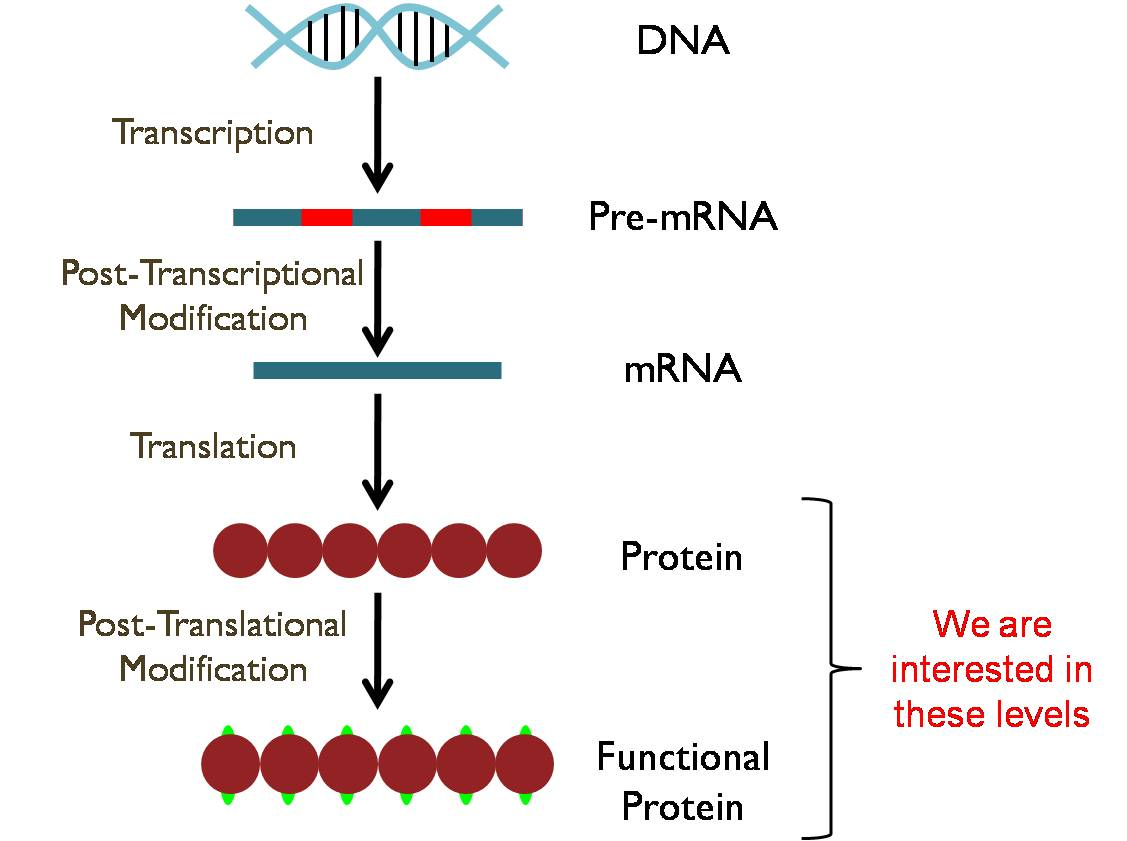
\includegraphics[scale=0.55]{image/processes.jpg}}
\caption{Basic biological processes of producing functional proteins from DNA.}
\label{fig:processes}
\end{figure}

The proteome is the entire complement of proteins expressed by the genome in a cell or tissue or bio-fluid of an organism at a given time point under a well-defined set of conditions \citep{Boehm2007}. A protein's function corresponds to when and where it is expressed. Hence, identification and localisation of many more unknown  proteins and their functions is the ultimate goal of proteomic research. 

There are many ways to study proteins. For example, a protein's physical structure can be studied by X-ray crystallography~\citep{Blow2002}, protein-protein interactions are studied by the yeast two-hybrid system~\citep{Fields1989}, and the abundance of an individual protein under a defined condition can be studied using isotopic-labelling. The latter is also referred to as \emph{quantitative proteomics}. 

The biological objective of this thesis is to identify the proteins in a set of target samples, namely the inner and outer LV from healthy and diabetic rats, and measure their relative abundances using MudPIT in conjunction with iTRAQ\textsuperscript{TM}, a type of isotopic-labelling. This information will subsequently be used to infer differential protein abundance between the inner and outer LV of healthy and diabetic rat populations.

\subsection{Multi-dimensional Protein Identification Technology} \label{sec:MudPIT}
MudPIT refers to the process of separating a protein complex or peptide mixture, using the different properties of amino acids, into usually three orthogonal dimensions~\citep{Washburn2001}. Typically, the first separation is by charge, using \emph{strong cation exchange chromatography} (SCX), followed by hydrophobicity, using \emph{reversed phase liquid chromatography} (RPLC). The third dimension of separation is by mass and is carried out by \emph{mass spectrometry} (MS). This reduces the sample complexity and enables high throughput protein analysis. Hence, each  MudPIT \emph{run} is comprised of these three steps of separation.

The SCX column contains immobilised negatively charged sulfonic acids which form an ionic interaction with the positively charged peptides. Hence, the charge separation by SCX divides a protein digest, (i.e. a mixture of peptides), into many different fractions based on the strength of charge interaction between the peptides and sulfonic acids. Different peptide sequences will have different affinities for the SCX resin. This allows for complex peptide mixtures to be fractionated by gradually increasing the concentration of a competing salt solution (for binding to the sulfonic acid groups in a gradient) in a step-wise manner. The range of the salt concentration is between 10mM to 500mM. Hence, at each interval of salt concentration, a set of peptides is released to move into the next MudPIT phase. Each of these charge intervals is referred to as a \emph{salt step}, and increasing the number of salt steps permits the detection of proteins having low abundance. Ten salt steps were used for our experiment.

The set of peptides from each charge fraction are then separated by RPLC based on hydrophobicity. This is achieved with a separate column which contains silica beads with chains of 18 carbon atoms attached. The peptides are loaded into the column resulting in hydrophobic interactions with the carbon chains. An organic solvent is then added to the column in concentrations that increase over time, causing the peptides to emerge or \emph{elute} from the column, with the least hydrophobic peptides eluting first. Eluted peptide are then detected in the mass spectrometer.

The mass analysis is performed by MS whereby each peptide's \emph{mass-to-charge ratio} (m/z) is measured and, from which, the molecular mass is calculated. A more detailed description of peptide separation can be found in \cite{Eidhammer2008}. 

\emph{Tandem mass spectrometry} (MS/MS), which consists of two repeated phases of MS, was used for this study. Peptide fragmentation occurs between the two phases of MS and, hence, identification and quantification of the peptides and proteins is based on these peptide fragments. MS/MS enables a higher specificity in protein identification and allows for more accurate quantification.

There are some limitations associated with MudPIT. The variation in signal intensity between different MudPIT runs can be large, making the comparisons of peptide or protein abundances between samples difficult. This limitation has been resolved with the introduction of iTRAQ\textsuperscript{TM} labelling which enables the simultaneous analysis of up to eight distinct protein digests within a single MudPIT run.

\subsection{iTRAQ\textsuperscript{TM} for Protein Quantitation}\label{sec:iTRAQ}
In its initial format, introduced by \cite{Ross2004}, iTRAQ comprised of four isobaric tags, each consisting of a reporter group, a balance group and a peptide reactive group. The reactive group binds the N-terminus at the start of each peptide, and, if the peptide contains lysine residues (i.e. amino acid) then, also on the lysine's side chain. The m/z values of the four reporter groups range in value from 114 to 117, with corresponding balance group values ranging from 31 to 28, respectively. Thus, each of four tags has an identical total m/z value of 145, making them isobaric. This enables identical peptide species, differentially labelled with the four tags, to be indistinguishable with respect to the intact mass of the peptide when selected for MS/MS~\citep{Ross2004}. For MS/MS, the relative abundances are determined from the reporter ion signals at m/z value of 114, 115, 116 and 117 on the \emph{mass spectrum}. A mass spectrum is a graphical representation of the peptides and peptide fragments based on their m/z value and abundances, and is generated for both phases of MS/MS. Thus, the four different labels allow four different samples to be simultaneously analysed~\citep{Ross2004}.
  
\begin{figure}[htb]
\centering{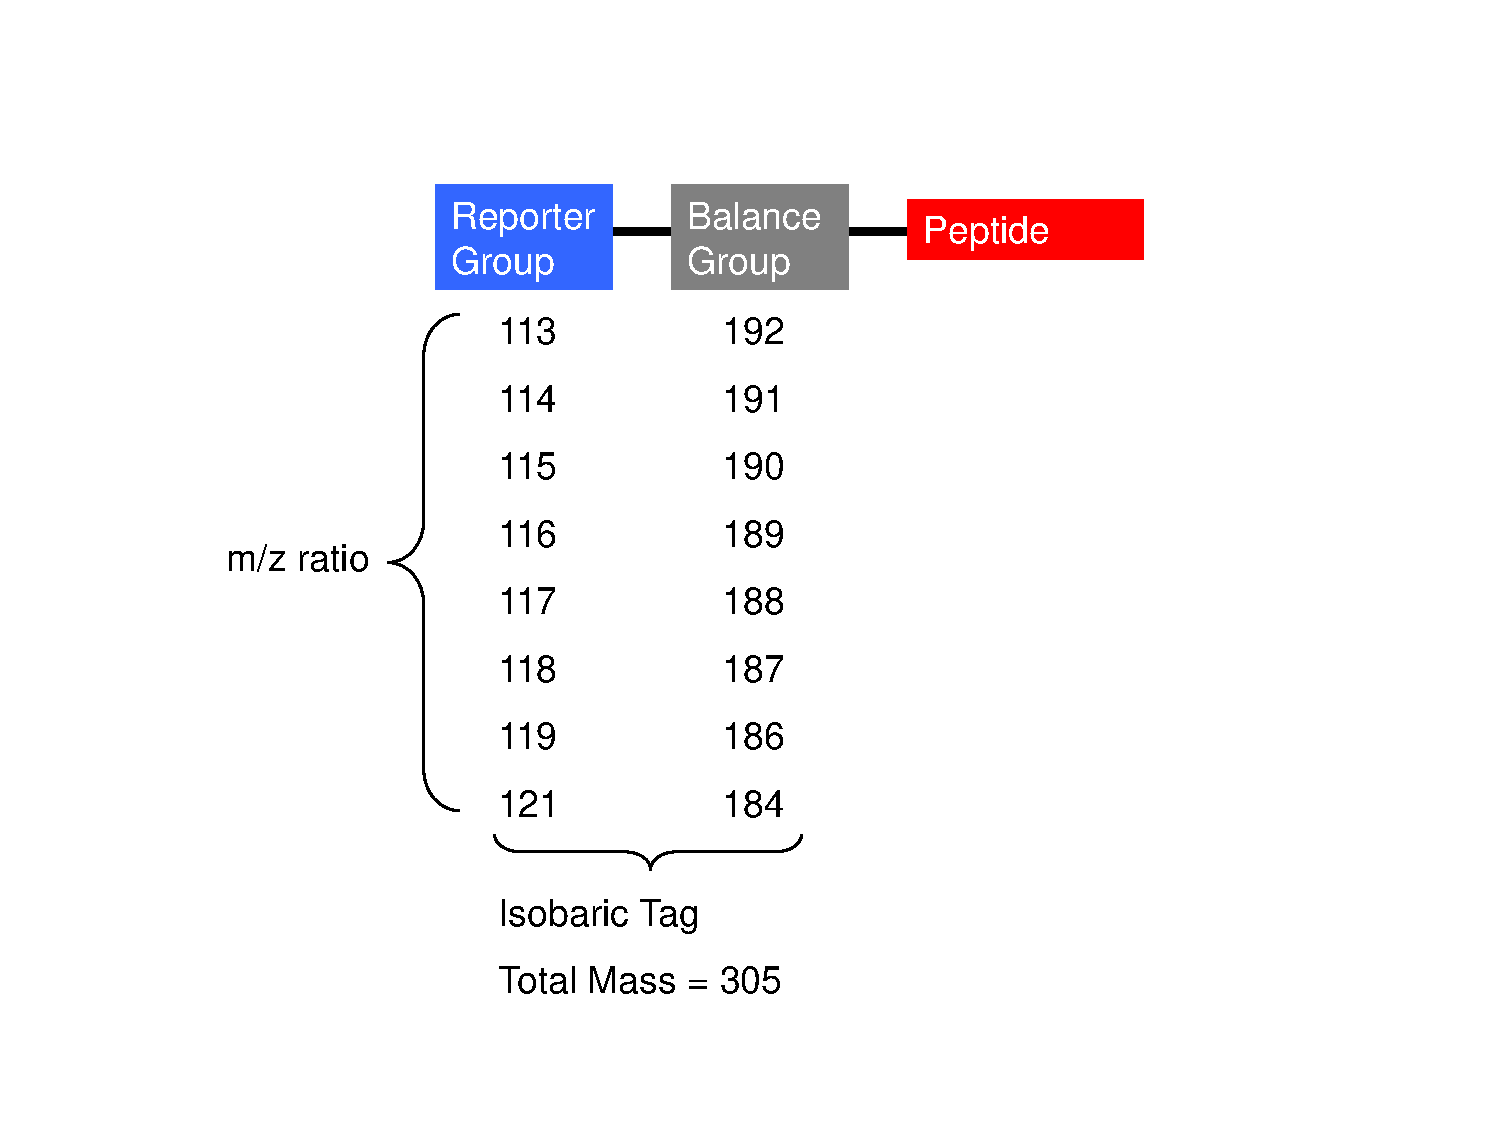
\includegraphics[scale=0.6]{image/iTRAQtags.pdf}}
\caption{Structure of 8-plex-iTRAQ\textsuperscript{TM} tags showing reporter and balance group masses measured in m/z~\citep{Choe2007}.}
\label{fig:8-plex}
\end{figure}

\cite{Choe2007} described a new multiplexing strategy, using the same concept as the four-plex iTRAQ\textsuperscript{TM} system, which allows the simultaneous analysis of up to eight distinct protein samples (see Figure~\ref{fig:8-plex}). This scheme has the reporter ion signals located at m/z values of 113, 114, 115, 116, 117, 118, 119 and 121. A label for an m/z of 120 is not used because this has the same mass as the phenylalanine immonium ion~\citep{Pierce2008}.   

\section{Overview}
The aim of this thesis is to develop a general theory in two-phase experiments. Chapter 2 describes the decomposition method for two-phase experiments with the construction the ANOVA table. As mentioned by \cite{Brien2011}, the ANOVA tables with the EMS for two-phase experiments are valuable in comparing the properties of different two-phase experimental designs. However, there is no any tool can automatically generate a such table. An R package called infoDecompuTE which stands for information decomposition of two-phase experiments is presented which allows the statistical researchers to quickly check the properties of the ANOVA table with EMS by entering any single or two-phase experimental design. This package will not only allow researchers to determine whether or not a valid F-test can be conducted, it will also enable them to study the decomposition of the raw data into different strata and sources of variation.

For a given set of design parameters, there are often many ways to allocate the samples collected from the Phase 1 experiment to the blocks in the Phase 2 experiment. Chapter 3 and 4 will show that the objective function defined can identifies the best allocation in terms of allowing a formal test of treatment effects to be conducted with the highest average efficiency factor. The objective function is optimised using a simulated annealing algorithm (SA). Chapter 3 and 4 will present objective functions for finding the optimal two-phase design, where the Phase 1 experiment is arranged in a completely randomised design and randomised block design, respectively. The Phase 2 experiment is in a randomised block design. In addition, an improved version of the SA, which is more efficient, is presented.

Finally, Chapter 5 describes the method in estimating the variance components and the effective degrees freedom (EDF) for the two-phase experiments. The restricted maximum likelihood method is described in estimating the variance components form the two-phase experiment with non-orthogonal block structures. EFD, for different possible values of the variance component estimates, will be used to compare the different optimal Two-phase design found from Chapter 3 and 4. These specific examples will be used to elucidate the properties of different candidate designs and to work towards a general theory.  


\bibliographystyle{apalike}
\bibliography{Reference/ref}

\end{document}
